\chapter{Event Reconstruction}
\label{sec:Reconstruction}

The reconstruction is the last stage of the data preparation and is the same for both genuine detector data and MC samples. The reconstruction process aims to interpret the output of the detector and to guess which particle could cause such response. Different analyses requires different focus on different types of particles, and because of that there are many reconstruction algorithms which make emphasis on different aspects of particles behavior. There are also several groups in ATLAS each of them is working on the algorithms for certain group of particles. For \Zee\ analysis the electrons are used, and the group studying the details of the electron and photon reconstruction is called "e/gamma". The group suggested several algorithms for the reconstruction of the both electrons and photons. The photons are not very important for \Zee\ analysis (although the study of the photons can improve the background estimation for the \Zee\ process, for this analysis it was not done), whereas the algorithms for electrons will be highlighted in this chapter. In section~\ref{sec:Rec_elec} the reconstruction algorithms itself will be described, while in sections~\ref{sec:Rec_elecID} and~\ref{sec:Rec_eleciso} there will be descriptions of methods to increase the quality of the reconstruction.

\section{Electron reconstruction}
\label{sec:Rec_elec}

There are several algorithms that are used to reconstruct the EM-particles (electrons and photons), each of them reconstructs its own set of particles for every event. To distinguish which particle was reconstructed by what algorithm, the "author" field was introduced. The field consists of 5 bits each of them can be 1 or 0 depending on whether the corresponding algorithm reconstructed that particular particle (one particle can be reconstructed by more than one algorithm). The field is then interpreted as decimal integer. The list of algorithms is as follows:
\begin{itemize}
\item {\bfseries AuthorElectron} Electron reconstructed by standard cluster-based algorithm. It requires both EM cluster and a matching track.
\item {\bfseries AuthorSofte} Electron reconstructed by the track-based algorithm. This algorithm doesn't require EM cluster, only the track. This author can overlap with the previous.
\item {\bfseries AuthorPhoton} Photon reconstructed by standard cluster-based algorithm. Same as the first, only for photons.
\item {\bfseries AuthorFrwd} Electron reconstructed by the Forward cluster-based algorithm. As the inner detector doesn't provide tracks for $\eta > 2.5$, the algorithm for forward particles uses only the cluster, and is tuned to be used in the forward detectors.
\item {\bfseries AuthorRConv} Photon that is duplicated with electron. Is used to mark the special cases when both electron and photon reconstruction algorithms return positive for the same particle.
\item {\bfseries AuthorTrigElectron} and {\bfseries AuthorTrigPhoton} Mark the trigger particles. The triggers were discussed in Sec.~\ref{sec:ATLAS_trigger}.
\end{itemize}

Because of the much difference between the algorithms for central and forward electrons, the reconstruction process for both will be discussed separately.

\subsection{Central}

The central electron is the electron with $\eta < 2.5$. In this area of the detector both EM calorimeter and tracker are present, so the reconstruction algorithms can make use of both. In the central region there are two  EM calorimeters: EMB and the outer ring of the EMEC, and the standard cluster-based algorithm behave slightly different in them. In current analysis only the central electrons reconstructed by the standard algorithm were used, so only it will be described. It consists of three main stages~\cite{lib:elec_reco}: the initial search for a EM-cluster, the track matching and the final reconstruction of the electron candidate. For the initial search the sliding-window algorithm is used with the size of $3 \times 5$ cells in units of $0.025 \eta \times 0.025 \varphi$ each. The seeding energy threshold for the algorithm is 2.5 GeV, and from the MC calculation of W and Z decays, the efficiency is expected to be about 97\% at $E_{t} = 7$ GeV and almost 100\% at $E_{t} > 20$ GeV. During the second stage every cluster is matched with a track reconstructed from the tracker. The reconstruction of the track is pretty straightforward: it is seeded by the hit in the innermost layer of the tracker, and then propagated outside by connecting the closest hit of the adjacent layer~\cite{lib:track_reco}. The matching algorithm tries to find the track with the impact point within of $|\Delta\eta| < 0.05$ and $|\Delta\varphi| < 0.1$. The size of $\Delta\varphi$ is taken bigger to account for the possible bremsstrahlung losses during the pass of the solenoidal magnetic field. If there are several such tracks, the closest one is chosen, with the priority given to the tracks with the hits in pixel detector or SCT (as opposed to the TRT, see section~\ref{sec:ATLAS_tracker}). If no track can be found, the candidate is classified as a photon, and the photon-reconstruction algorithm is used for it. The final stage is the calculation of the cluster energy and other cluster variables. It is during this stage, when the differences between EMB and EMEC come into play. The size of the window differs for these two detectors: it is $3 \times 7$ cells in EMB and $5 \times 5$ in EMEC in the same units of $0.025 \eta \times 0.025 \varphi$. The $\eta$ and $\varphi$ spatial coordinates of the electron are taken from the matched track at the interaction vertex, the energy is calculated from the cluster. Still, all the variables from both cluster and matched track are saved and available separately for the needs of the analysis.

\subsection{Forward}

The forward region of the calorimeter starts from $\eta = 2.5$ and includes two detectors: the inner wheel of the EMEC and FCAL. There is no tracker in this region, so the reconstruction algorithm deals only with clusters. Because of this the reconstruction algorithm can't make a difference between electrons and photons, and electrons and positrons. For this region another cluster-construction algorithm is used which is called "topological clustering"~\cite{lib:elec_reco_fwd}. This algorithm is very effective at noise suppression, which is very important for forward region. The algorithm is seeded by a single cell with an energy significance which is above a high signal to noise ratio threshold. Then the cluster is expanded by adding the neighbor cells with the said ratio being above the medium threshold, and then finalized by taking in all the cells above low threshold. The standard configuration for this algorithm for EM calorimeters is called "EM~633", with the thresholds being 6, 3 and 3 respectively. If the process of cluster expanding proceeds to the hadron calorimeter, the configuration "Had~420" is used. The spatial coordinates of the reconstructed electron is then calculated as a barycenter of the cluster. This algorithm produces the variable-sized cluster, as opposed to the sliding-window algorithm, which produces a cluster with a fixed size. Because of the three-dimensional nature of the cluster expanding used in the algorithm, it is very effective in suppressing the pileup. The effectiveness in terms of electron reconstruction is predicted (via MC simulation) to be above 99\% for the electrons with $E_{t} > 20$ GeV. To be reconstructed, the electron candidate must have $E_{t} > 5$ GeV, and have no significant energy deposits in the hadron calorimeter.

\section{Electron identification}
\label{sec:Rec_elecID}

The electron identification is the next step of the data preparation, and is aimed to reduce the number of false-positive cases of the reconstruction algorithms such as background hadrons from semileptonic decays or photon conversions. The identification is implemented using several cuts on cluster, track, and combined cluster-track variables. For use in the analysis, three sets of cuts were introduced, with every consecutive being a superset of the predecessor. These sets are named loose, medium and tight. Each one of them is more effective in background suppression than the previous, but is less effective in terms of identification efficiency, which is they increase the amount of false-negative cases.

The description of these identification criteria is described below.
\begin{itemize}
\item {\bfseries Loose}: This is the least demanding criteria, that performs only a basic cuts on the reconstructed electron candidate. It takes into account the shower shape variables from the EM calorimeters and the hadronic leakage information. The most important shape variables can be seen in Fig.~\ref{fig:REC_shower_shapes}, and they usually show the fracture of the energy deposited in some parts of the cluster (in the beginning, and the end, in the center etc), relative to the whole energy of the cluster. The distributions usually have peaks, where the "good" electrons are located, and tails, with "bad" electrons. The thresholds for each variable is picked experimentally. The criteria also increases the requirements on the quality of the track and of the track-cluster matching. It improves the rejection of the hadronic background by a factor of $\sim 5$ in the range $30 < E_{t} < 40$ compared to the bare reconstruction algorithms, while not affecting the identification efficiency.
\item {\bfseries Medium}: This is an overall a more demanding version of the "loose" criteria, with a more demanding requirements on the same variables. It also introduces several new requirements, mostly on the track, the most important one being the requirement of the hit in the innermost layer of the tracker, which aims to suppress the photon conversion background. It is $\sim 10$ times more efficient in background rejection than "loose", but has a drawback of having a worse identification efficiency.
\item {\bfseries Tight}: This one makes a full use of all the identification tools available. In addition of more strict requirements for every variable used in "medium", it also makes new: on the track extension in the TRT and on the ratio between track momentum and cluster energy. It also takes into account the list of reconstructed photon conversions associated with the same vertex. Overall, it increases the the background rejection by the factor of two with respect to "medium".
\item {\bfseries Forward Id}: For the forward region of the calorimeter, the identification criteria follow the similar pattern as for the central region, because of lack of the tracking information, only the shower parameters are taken into account. The shower shape, the longitudal, transverse and normalized lateral momenta are all used for the identification process. In 2011, the pileup increased drastically for the forward region, so the criteria became more strict, and are derived from the previous data. The thresholds come in four bins based on the number of primary vertexes reconstructed in the event ($N_{PV} = 1-3$, $4-6$, $7-10$, $>10$). All the three criteria use the same set of variables, but progressively increase the thresholds, with the {\itshape fwdTight} rejection factor being 2 to 3 times bigger than the {\itshape fwdLoose} one.
\end{itemize}

The criteria for the forward electrons are different, since the forward region lacks the tracker, and has a significantly higher pileup. The cuts are applied to the cluster itself, and take into account such parameters as longitudinal second momentum, transverse second momentum, normalized lateral momentum and so on. The fact that the reconstruction algorithm for forward region produces a three-dimensionally shaped cluster helps greatly. The loose, medium and tight criteria are also defined for the forward region, but work on the same variables, only with consecutively stricter requirements.

For 2011 the new set was introduced which was attuned more attuned to the data and was more effective at background-suppression. The new set was called "IsEM++" criteria (the previous was called just "IsEM"), and consist respectively of loose++, medium++ and tight++. The difference between the sets is mostly the tunes to the variables thresholds.

\begin{figure}
\center{
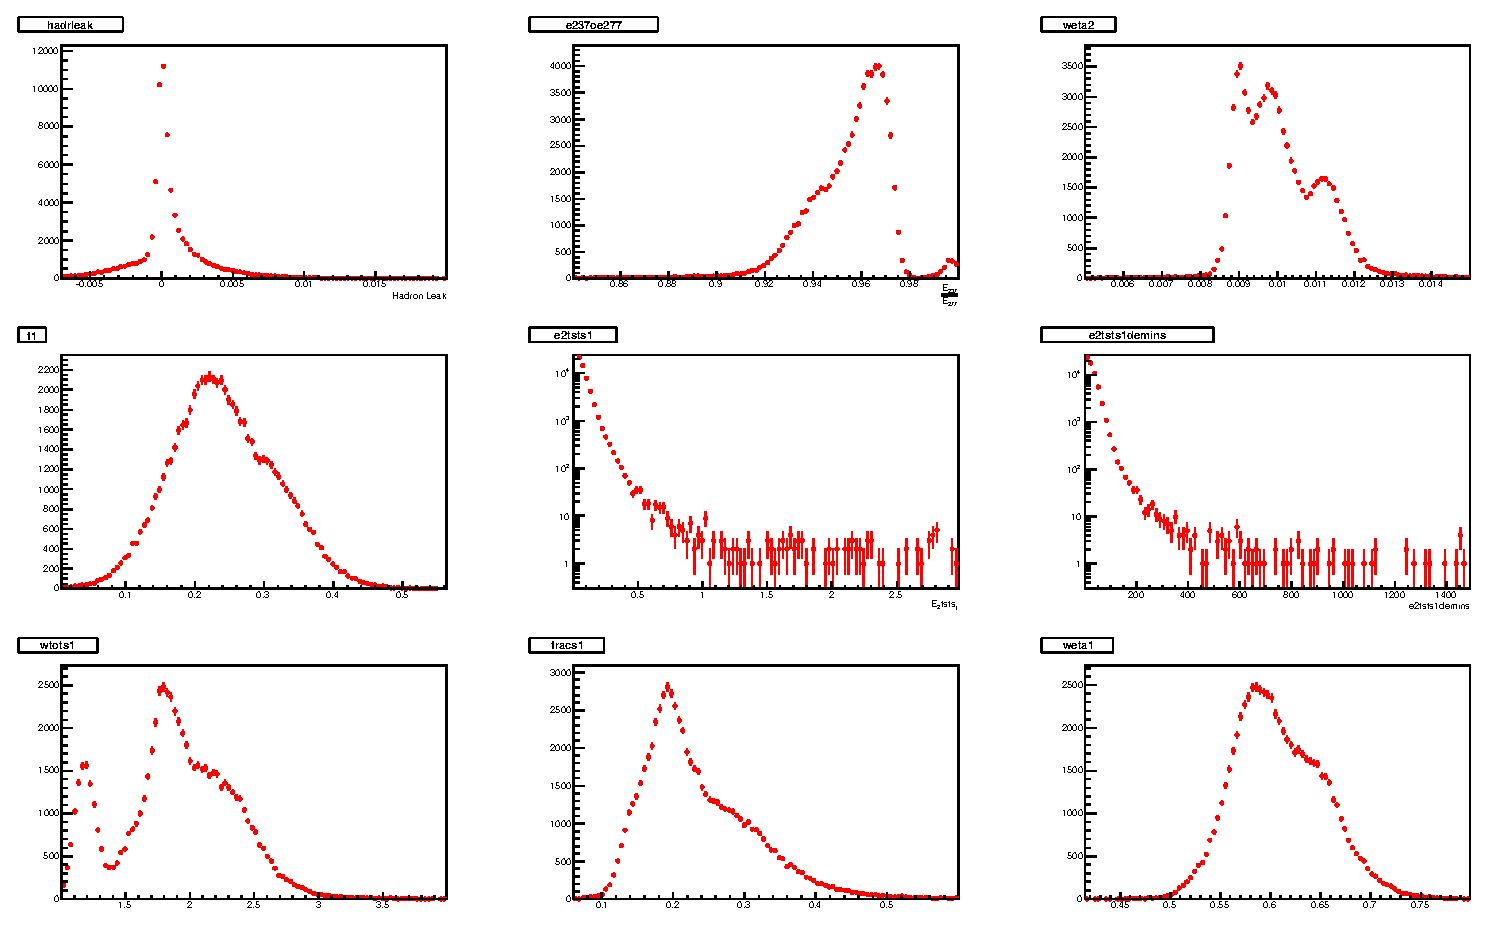
\includegraphics[width=1.0\textwidth]{figures/REC_shower_shapes.eps}
\caption{Some of the shower shapes variables shown for MC-simulated electrons. All of these variables are used for the electron identification in the central region.\tbu A BETTER PLOT}
\label{fig:REC_shower_shapes}}
\end{figure}

\section{Electron isolation}
\label{sec:Rec_eleciso}

To further suppress fake electron background, the isolation check is also used. The isolation check relies on Etcone variable, which is the sum of the energy in a cylinder surrounding the cluster, excluding the cluster itself. Although we use the cylinder, in a sense that it is a round shape with a constant $\Delta R$ where $\Delta R = \sqrt{\Delta\eta^{2} + \Delta\varphi^{2}}$, in real geometry it looks like a cone, that's why all the names of the isolation variables contain "cone".  The radius of the cylinder that was used is written in the name of the variable, so there are several of them, e.g. Etcone20, Etcone40, etc, where 20 or 40 means $\Delta R = 0.20 , 0.40$~\cite{lib:reco_iso}. The Etcone variable can use cluster $E_{t}$ as well as track $E_{t}$, and different isolation criteria use one or another or both. The said criteria is just the cut on the ratio of the Etcone energy to the cluster energy. If the ratio is low, we are dealing with the high-isolation electron. This is the best-case scenario. The higher values of the ratio means low-isolation electron, the high error in energy reconstruction is expected for this kind of electrons. The high value of the ratio means that the electron is most likely a fake: a misidentified muon or hadron jet with a mismatched track.

For \Zee\ central-forward analysis, the isolation cuts named Iso98 for Etcone20 and Iso97 for Ptcone40 were used for the central electron. It allowed to reduce the background to the factor of 2, while still retaining the electron efficiency of 97-98\%.
